\documentclass[addpoints,spanish, 12pt,a4paper]{exam}
%\documentclass[answers, spanish, 12pt,a4paper]{exam}
\printanswers
\pointpoints{punto}{puntos}
\hpword{Puntos:}
\vpword{Puntos:}
\htword{Total}
\vtword{Total}
\hsword{Resultado:}
\hqword{Ejercicio:}
\vqword{Ejercicio:}

\usepackage[utf8]{inputenc}
\usepackage[spanish]{babel}
\usepackage{eurosym}
%\usepackage[spanish,es-lcroman, es-tabla, es-noshorthands]{babel}


\usepackage[margin=1in]{geometry}
\usepackage{amsmath,amssymb}
\usepackage{multicol}
\usepackage{yhmath}

\pointsinrightmargin % Para poner las puntuaciones a la derecha. Se puede cambiar. Si se comenta, sale a la izquierda.
\extrawidth{-2.4cm} %Un poquito más de margen por si ponemos textos largos.
\marginpointname{ \emph{\points}}

\usepackage{graphicx}

\graphicspath{{../img/}} 

\newcommand{\class}{2º Bachillerato CCSS}
\newcommand{\examdate}{\today}
\newcommand{\examnum}{Recuperación 1ªEv.}
\newcommand{\tipo}{A}


\newcommand{\timelimit}{50 minutos}

\renewcommand{\solutiontitle}{\noindent\textbf{Solución:}\enspace}


\pagestyle{head}
\firstpageheader{
\includegraphics[width=0.2\columnwidth]{header_left}}{\textbf{Departamento de Matemáticas\linebreak \class}\linebreak \examnum}{
\includegraphics[width=0.1\columnwidth]{header_right}}
\runningheader{\class}{\examnum}{Página \thepage\ of \numpages}
\runningheadrule


\usepackage{pgf,tikz,pgfplots}
\pgfplotsset{compat=1.15}
\usepackage{mathrsfs}
\usetikzlibrary{arrows}


\begin{document}

\noindent
\begin{tabular*}{\textwidth}{l @{\extracolsep{\fill}} r @{\extracolsep{6pt}} }
\textbf{Nombre:} \makebox[3.5in]{\hrulefill} & \textbf{Fecha:}\makebox[1in]{\hrulefill} \\
 & \\
\textbf{Tiempo: \timelimit} & Tipo: \tipo 
\end{tabular*}
\rule[2ex]{\textwidth}{2pt}
Esta prueba tiene \numquestions\ ejercicios. La puntuación máxima es de \numpoints. 
La nota final de la prueba será la parte proporcional de la puntuación obtenida sobre la puntuación máxima. 

\begin{center}


\addpoints
 %\gradetable[h][questions]
	\pointtable[h][questions]
\end{center}

\noindent
\rule[2ex]{\textwidth}{2pt}

\begin{questions}


\question Sea la matriz: $A=\left[\begin{matrix}1 & 0 & 1\\2 & 1 & 1\\1 & 0 & a^{2}\end{matrix}\right]$, con $a$ un parámetro real:
%\noaddpoints % to omit double points count

\begin{parts}
\part[1] ¿Para qué valores del parámetro $a$ el sistema de ecuaciones $$A\cdot \left[\begin{matrix}x\\y\\z\end{matrix}\right]=\left[\begin{matrix}0\\0\\0\end{matrix}\right]$$ tiene solo la solución: $\begin{matrix}x=0 & y=0 & z=0\end{matrix}$ ?
\begin{solution}
$\left[\begin{matrix}1 & 0 & 1 & 0\\2 & 1 & 1 & 0\\1 & 0 & a^{2} & 0\end{matrix}\right] \to \left[\begin{matrix}1 & 0 & 1 & 0\\0 & 1 & -1 & 0\\0 & 0 & a^{2} - 1 & 0\end{matrix}\right] \to det(A)= a^{2} - 1 \to det(A)= \left(a - 1\right) \left(a + 1\right)$. \\ \\ Discusión: \\Si a $\neq\left[ -1, \  1\right]\to $ S.C.D. \\Si a=-1: \\ $\left[\begin{matrix}1 & 0 & 1 & 0\\0 & 1 & -1 & 0\\0 & 0 & 0 & 0\end{matrix}\right] \to ran(A^*)=2 \land ran(A)=2 \to$  S.C.I.\\ \\  Si a=1: \\ $\left[\begin{matrix}1 & 0 & 1 & 0\\0 & 1 & -1 & 0\\0 & 0 & 0 & 0\end{matrix}\right] \to ran(A^*)=2 \land ran(A)=2 \to$  S.C.I.

\end{solution}

\part[2] Para $a=-1$, determina justificadamente y sin resolverlo cuántas soluciones tiene el sistema $$A\cdot \left[\begin{matrix}x\\y\\z\end{matrix}\right]=\left[\begin{matrix}1\\1\\1\end{matrix}\right]$$
\begin{solution}
Para a=$1$: \\ $\left[\begin{matrix}1 & 0 & 1 & 1\\2 & 1 & 1 & 1\\1 & 0 & 1 & 1\end{matrix}\right] \to \left[\begin{matrix}1 & 0 & 1 & 1\\0 & 1 & -1 & -1\\0 & 0 & 0 & 0\end{matrix}\right] \to ran(A^*)=2 \land ran(A)=2 \to$  S.C.I.
\end{solution}

\part[1] Resuelve justificadamente el sistema del apartado anterior
\begin{solution}
Para a=$1$: \\ $\left[\begin{matrix}1 & 0 & 1 & 1\\2 & 1 & 1 & 1\\1 & 0 & 1 & 1\end{matrix}\right] \to \left[\begin{matrix}1 & 0 & 1 & 1\\0 & 1 & -1 & -1\\0 & 0 & 0 & 0\end{matrix}\right] \to \left\{\left( 1 - z, \  z - 1, \  z\right)\right\}$
\end{solution}


\end{parts}
\addpoints

\question Una empresa de carpintería tiene dos fábricas A y B en las que produce sillas, mesas y 
taburetes, y tiene que decidir el número de horas de trabajo en cada una de las dos fábricas para la semana 
próxima. Por cada hora de trabajo de la fábrica A, se producen 1 silla, 2 mesas y 4 taburetes, por cada hora 
de trabajo de la fábrica B se producen 4 sillas, 3 mesas y 2 taburetes. Durante la semana próxima la 
empresa tiene que producir, al menos, 80 sillas, 120 mesas y 96 taburetes. El coste por cada hora de 
trabajo de la fábrica A es de 1500 euros, mientras que el coste por cada hora de trabajo de la fábrica B es 
de 1000 euros. 

\begin{parts}
\part[2] Plantear un problema de programación lineal para determinar el número de 
horas que tiene que trabajar cada una de las fábricas para minimizar el coste.
\part[1] Resolver un problema de programación lineal para determinar el número de horas que tiene que trabajar cada una de las fábricas para minimizar el coste. ¿Cuál es el valor de ese coste 
mínimo?

\end{parts}
\begin{solution}
$$\left\{\begin{matrix}
x  \geqslant  0\\
y  \geqslant  0\\
x + 4y  \geqslant  80\\
2x + 3y  \geqslant  120\\
4x + 2y  \geqslant  96 \\
\end{matrix}\right.$$ 
\\
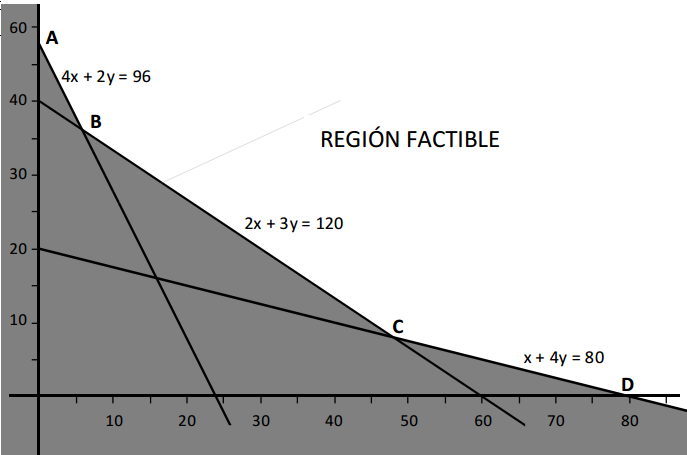
\includegraphics[scale=0.5]{re1_1} 
\\Vértices:\\
$A(0 , 48) \to f( 0 , 48)= 1500 \cdot 0 +  1000 \cdot 48 = 48000$\\
$B( 6,36) \to f( 6,36)=1500 \cdot 6 +  1000 \cdot 36 =  45000$\\
$C(48,8) \to f(48,8)=1500 \cdot 48 +  1000 \cdot 8 = 60000$\\
$D( 80 , 0) \to f( 80 , 0)=1500 \cdot 80 +  1000 \cdot 0 = 120000$\\

Por lo tanto, el coste mínimo, de 45000 euros, se obtiene al trabajar 6 horas la fábrica A y 36 horas la fábrica B.
\end{solution}

\question Para la compra de un artículo de precio 21,50 euros se utilizan monedas de 1 euro, de 50 céntimos de euro y
de 2 euros. El número total de monedas excede en una unidad al triple de monedas de 1 euro. El 30
\% de la suma del número de monedas de 1 euro con el doble del número de monedas de 50 céntimos coincide
con el número de monedas de 2 euros.
\begin{parts}
\part[2] Plantea un sistema de ecuaciones que refleje el enunciado
\part[1] Resuelve el problema
\end{parts}
\begin{solution}
$\left\{\begin{matrix}100 x + 50 y + 200 z = 2150\\x + y + z = 3 x + 1\\30 x + 60 y = 100 z\\\end{matrix}\right.$ \\  Por Gauss: \\ $\left[\begin{matrix}100 & 50 & 200 & 2150\\-2 & 1 & 1 & 1\\30 & 60 & -100 & 0\end{matrix}\right]\rightarrow\left[\begin{matrix}100 & 50 & 200 & 2150\\0 & 2 & 5 & 44\\0 & 0 & - \frac{545}{2} & -1635\end{matrix}\right]\to$ Sol:$\left\{\left( 6, \  7, \  6\right)\right\}$ \\ Por Matriz inversa: \\ $X=A^{-1}\cdot b=\left[\begin{matrix}\frac{8}{2725} & - \frac{34}{109} & \frac{3}{1090}\\\frac{17}{5450} & \frac{32}{109} & \frac{1}{109}\\\frac{3}{1090} & \frac{9}{109} & - \frac{2}{545}\end{matrix}\right]\cdot\left[\begin{matrix}2150\\1\\0\end{matrix}\right]=\left[\begin{matrix}6\\7\\6\end{matrix}\right]$. \ Ya que $\left[\begin{matrix}100 & 50 & 200\\-2 & 1 & 1\\30 & 60 & -100\end{matrix}\right]\xrightarrow{traspuesta}\left[\begin{matrix}100 & -2 & 30\\50 & 1 & 60\\200 & 1 & -100\end{matrix}\right]\xrightarrow{adjunta}\left[\begin{matrix}-160 & 17000 & -150\\-170 & -16000 & -500\\-150 & -4500 & 200\end{matrix}\right]\xrightarrow{inversa}\left[\begin{matrix}\frac{8}{2725} & - \frac{34}{109} & \frac{3}{1090}\\\frac{17}{5450} & \frac{32}{109} & \frac{1}{109}\\\frac{3}{1090} & \frac{9}{109} & - \frac{2}{545}\end{matrix}\right]$. \\ Por Cramer: \\ $det(A)=-54500$ \ $\Delta_0$, $s_0$: $\left[ -327000, \  6\right]$ \ $\Delta_1$, $s_1$: $\left[ -381500, \  7\right]$ \ $\Delta_2$, $s_2$: $\left[ -327000, \  6\right]$ \ 
 \end{solution}

\question Considerar la ecuación matricial  $$X\left[\begin{matrix}2 & 2\\2 & a^{2} + a\end{matrix}\right]= 2 \left[\begin{matrix}2 & 1\\4 & 0\end{matrix}\right]$$, con $a$ un parámetro real: 
\begin{parts}
\part[1] ¿Para qué valores del parámetro $a$ existe una única matriz $X$ que verifica la ecuación anterior?
\begin{solution}
$det(A)=2 a^{2} + 2 a - 4=2 \left(a - 1\right) \left(a + 2\right) \to a \neq \left[ -2, \  1\right] $
\end{solution}

\part[1] Si es posible, resolver la ecuación matricial para $a = 1$
\begin{solution}
Para $a = 1$ la matriz $A$ no tiene inversa, luego no se puede resolver la ecuación
\end{solution}

%\part[1] Resolver el sistema para $a=2$


\end{parts}

\addpoints



\end{questions}

\end{document}
\grid
